% !TeX spellcheck = it
\documentclass[a4paper,11pt]{article}
\usepackage[utf8]{inputenc}
\usepackage{graphicx}
\usepackage{subcaption}
\graphicspath{{./images/}}
\begin{document}
\begin{titlepage}
   \begin{center}
       \vspace*{1cm}
 
       \textbf{THETA DEX}
 
       \vspace{0.5cm}
        Manuale d'uso
 
       \vspace{5cm}
 
       \textbf{Daniele Ferrarelli, Marco Ferri, Giuseppe Marseglia, Lorenzo Valeriani}
 
       \vfill
   \end{center}
\end{titlepage}

  \section{Primo avvio}
  In questa fase viene fatto il download delle immagini e l’inizializzazione dei dati, bisogna solo attendere il completamente dell’operazione. Solitamente ciò impiega meno di un minuto.
  \begin{figure}[h!]
    \centering
  \fbox{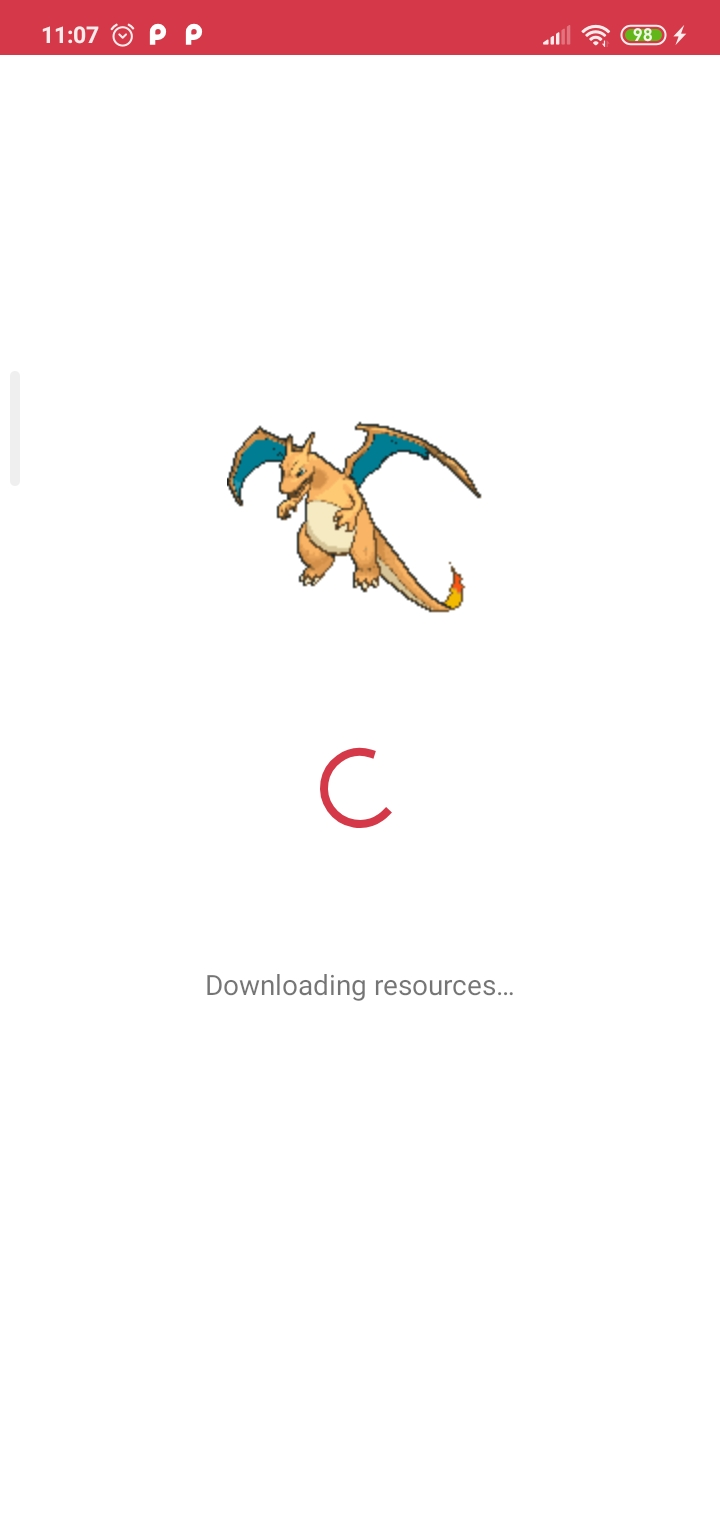
\includegraphics[width=150px]{loading.jpg}}
  \caption{Schermata caricamento iniziale.}
\end{figure}
\newpage

  \section{Schermata principale}
  \paragraph{}
  Questa è la schermata principale dell’applicazione. Da qui si può scorrere attraverso i vari elementi della lista.\\
Sulla destra, dopo un breve scorrimento della lista, è presente una barra per effettuare la navigazione in maniera più veloce.\\
  \begin{figure}[h!]
    \centering
  \fbox{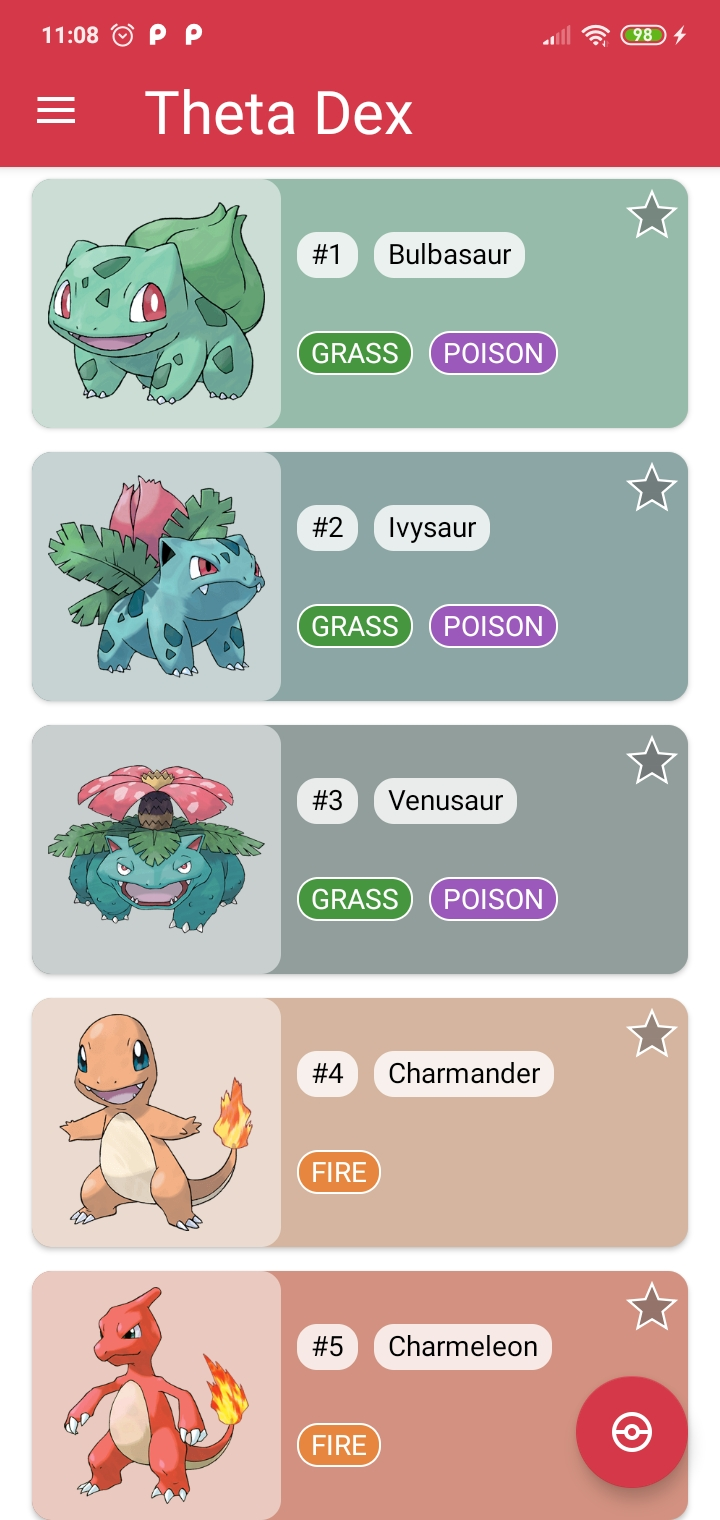
\includegraphics[width=150px]{home.jpg}}
	\caption{Schermata Home.}
\end{figure}
\newpage
In basso a destra è presente un bottone che racchiude diverse funzionalità. Al click rivela altri tre bottoni.\\Il primo apre una barra di ricerca che permette la ricerca sia tramite nome, anche solo la prima parte, e tramite ID. Se non è presente un Pokémon che rispetta i requisiti della richiesta, viene notificato tramite Toast.

Il secondo apre una carta che permette di filtrare in tempo reale i Pokémon per tipo. Ne accetta fino a due e non considera l’ordine in cui sono stati premuti. Se non è presente un Pokémon con la combinazione di tipi specificata, viene notificato tramite Toast.

Il terzo bottone permette di eliminare ogni filtro e/o ricerca, così da poter tornare alla vista del Pokédex contente tutti i Pokémon.

\begin{figure}[h!]
\fbox{
  \centering
  \begin{subfigure}[b]{0.3\linewidth}
    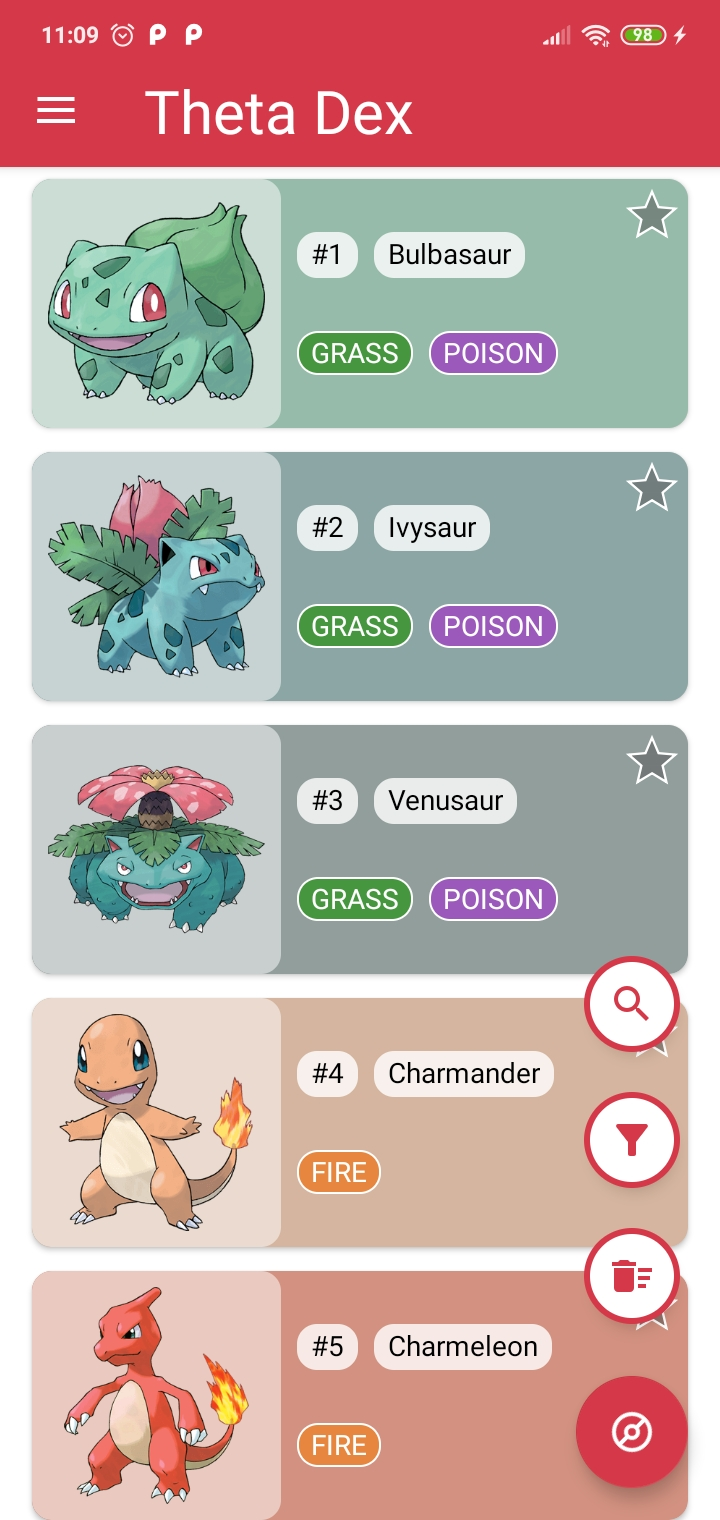
\includegraphics[width=\linewidth]{floating_button.jpg}
    \caption{Bottone Espanso.}
  \end{subfigure}
  \begin{subfigure}[b]{0.3\linewidth}
    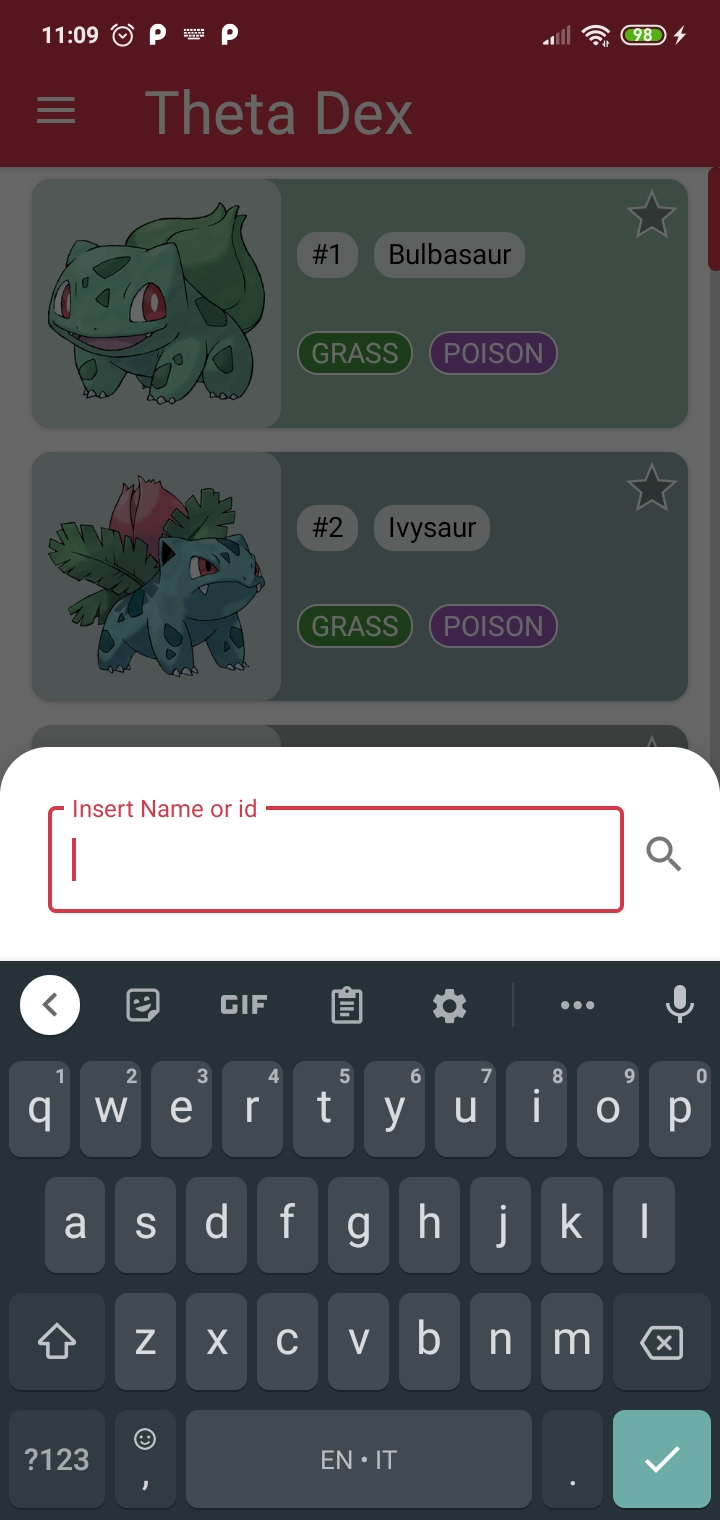
\includegraphics[width=\linewidth]{search.jpg}
    \caption{Schermata di ricerca.}
  \end{subfigure}
    \begin{subfigure}[b]{0.3\linewidth}
    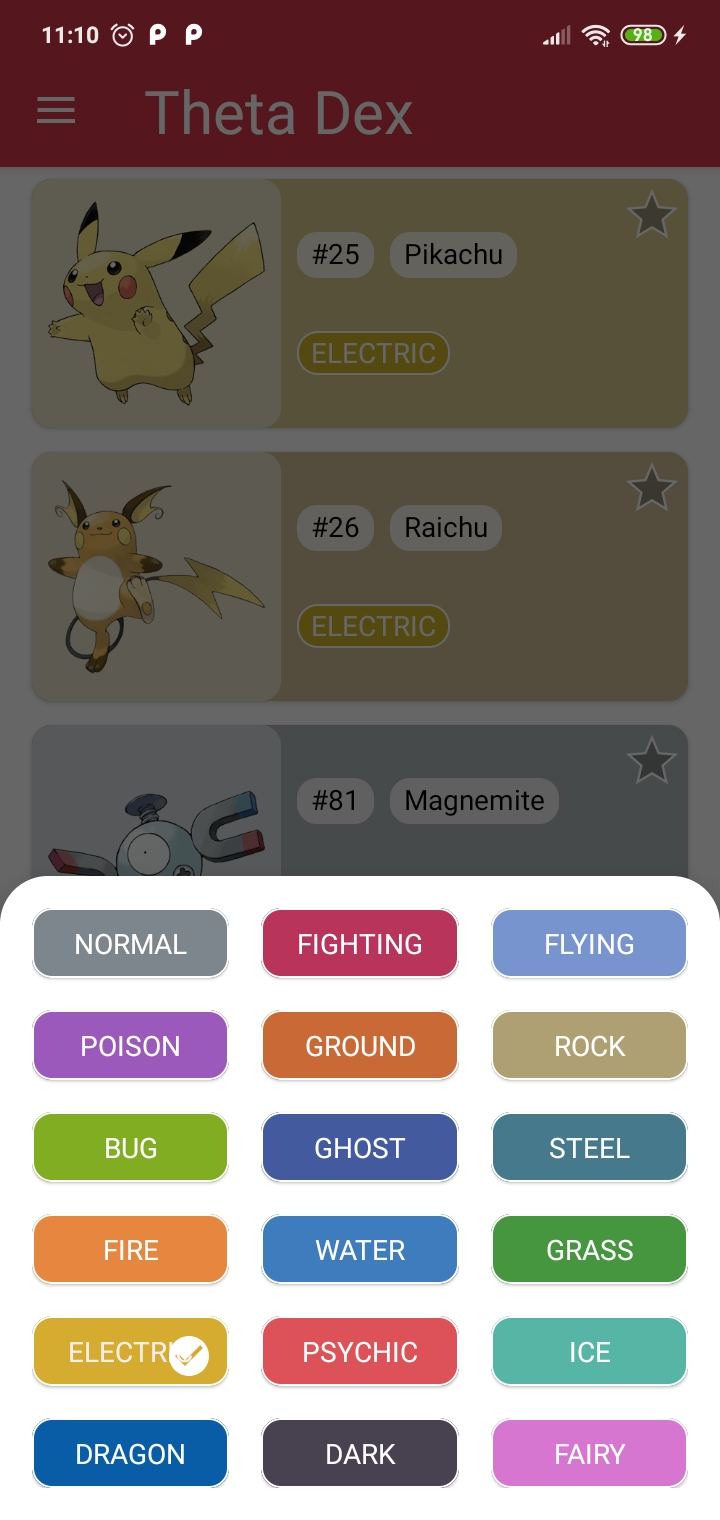
\includegraphics[width=\linewidth]{filter.jpg}
    \caption{Filtri.}
  \end{subfigure}
  \label{fig:home}
  }
\end{figure}
\newpage

\section{Menu}
Nelle schermate che non siano di dettaglio di un Pokémon, è presente in alto a sinistra che permetta l’apertura di un menu a comparsa laterale. Da questo ci si può muovere all’interno delle diverse schermate disponibili.
  \begin{figure}[h!]
    \centering
  \fbox{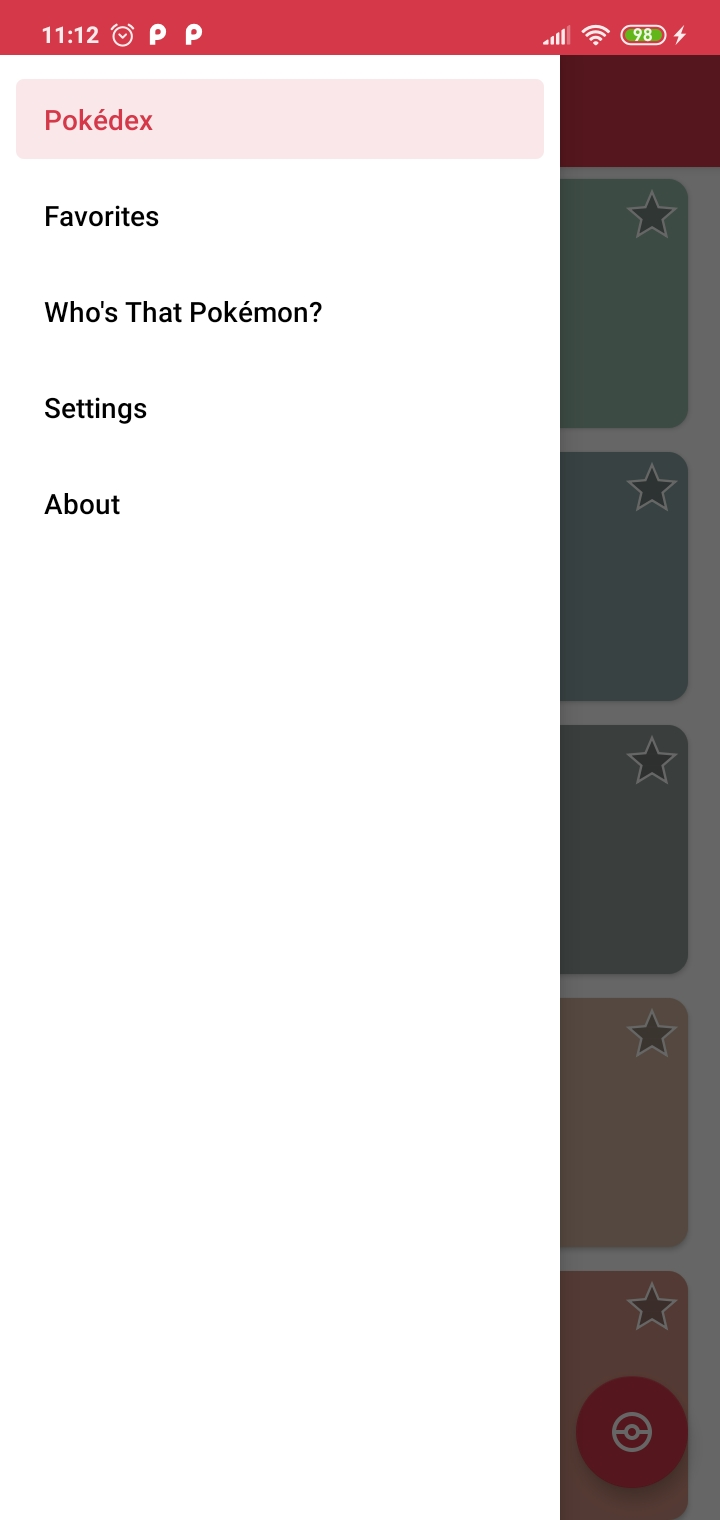
\includegraphics[width=150px]{menu.jpg}}
  \caption{Menu.}
\end{figure}
\newpage

\section{Preferiti}
    \subsection{Aggiunta ai preferiti}
  \paragraph{}
  Le carte dei Pokémon rispondono al click sull’icona della stella, al click sulla carta ed al click lungo sulla carta ed al in maniera differente.\\
Il click sulla stella permette di aggiungere o rimuovere un Pokémon dai preferiti.\\
Il click lungo sulla carta permette di entrare nella modalità di scelta multipla. Qui si possono selezionare fino ad un massimo di 10 Pokémon contemporaneamente.\\
Cliccando poi sull’icona dei tre puntini in alto a destra si possono compiere diverse azioni, quali: aggiungere i Pokémon selezionati ai preferiti, rimuovere i Pokémon selezioni dai preferiti o deselezionare tutto.\\
\begin{figure}[h!]
\fbox{
  \centering
  \begin{subfigure}[b]{0.3\linewidth}
    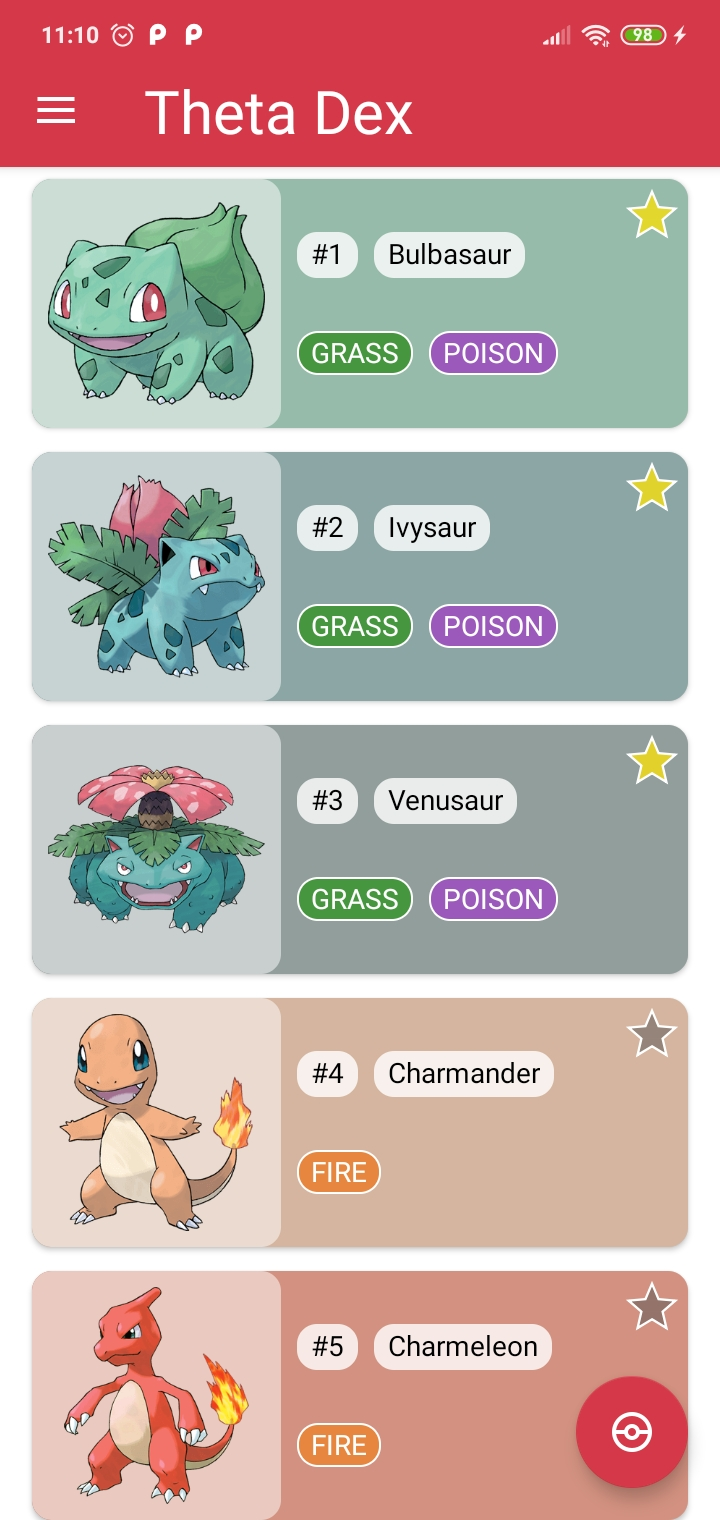
\includegraphics[width=\linewidth]{favorite_button.jpg}
    \caption{Schermata Home.}
  \end{subfigure}
  \begin{subfigure}[b]{0.3\linewidth}
    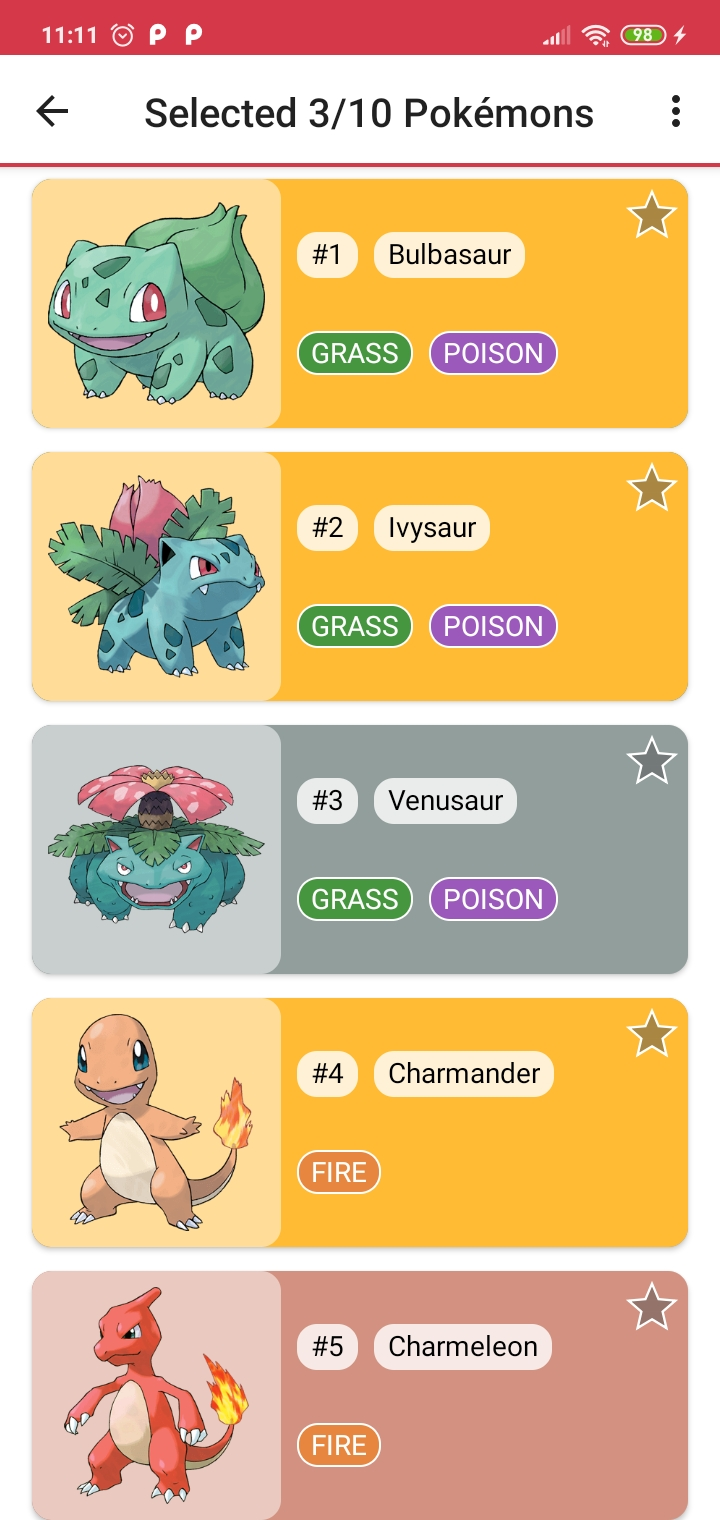
\includegraphics[width=\linewidth]{multiple_selection.jpg}
    \caption{Bottone Espanso.}
  \end{subfigure}
  \begin{subfigure}[b]{0.3\linewidth}
    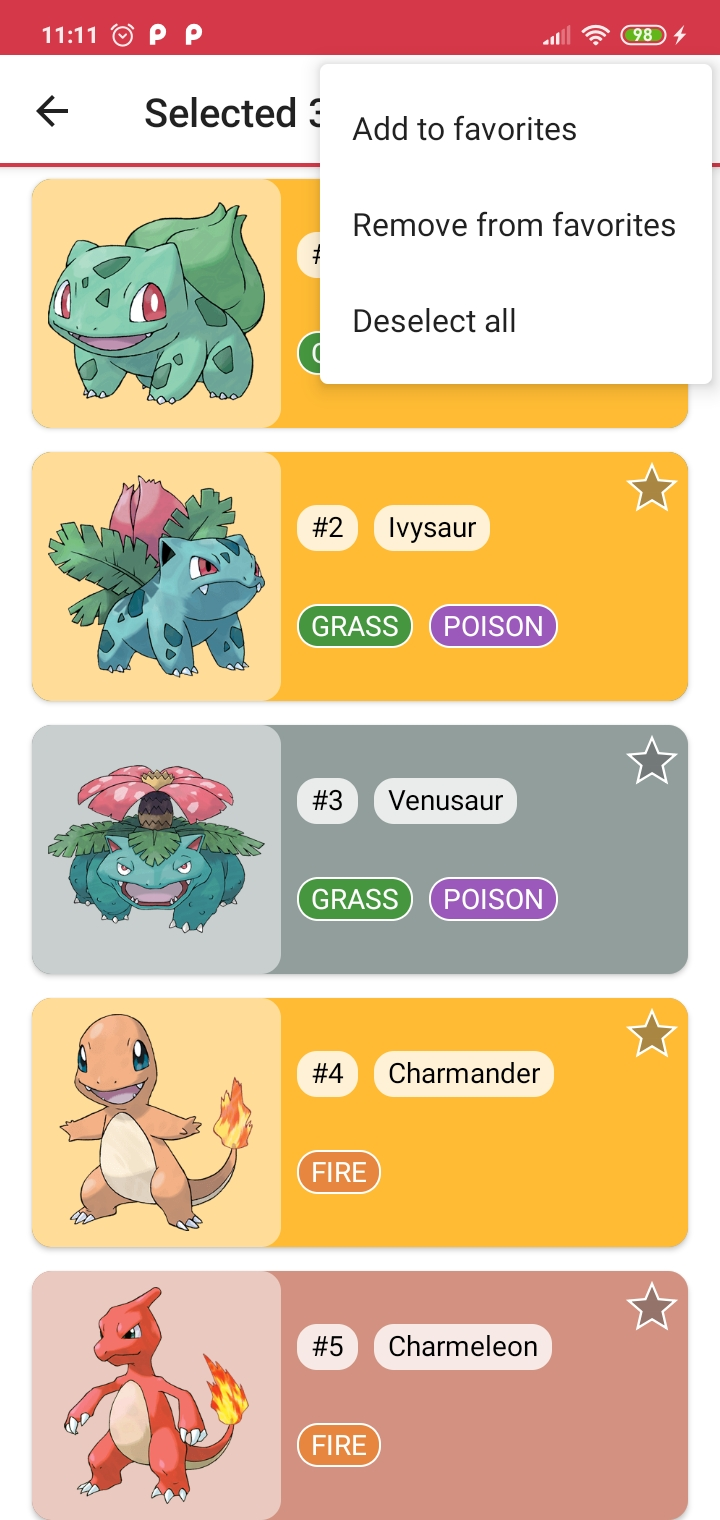
\includegraphics[width=\linewidth]{drop_down.jpg}
    \caption{Menu.}
  \end{subfigure}
  \label{fig:home}
  }
\end{figure}
\newpage

\subsection{Schermata dei preferiti}
La schermata dei preferiti è molto simile alla schermata principale del Pokédex. È raggiungibile dal menu laterale. Mostra solamente i Pokémon che sono stati aggiunti ai preferiti. Anche qui è possibile interagire con le carte dei Pokémon nelle stesse modalità della schermata principale.
  \begin{figure}[h!]
    \centering
\fbox{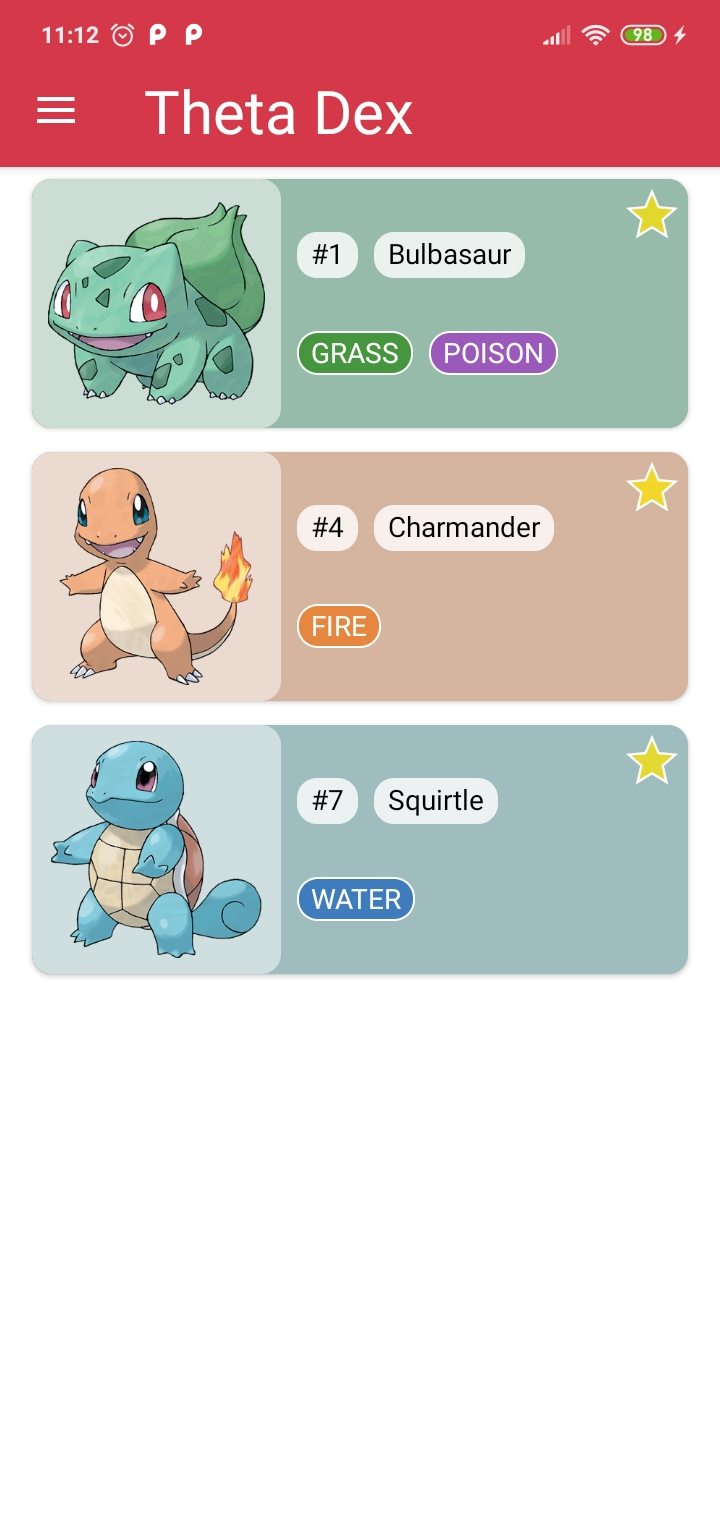
\includegraphics[width=150px]{favorite.jpg}}
  \caption{Schermata dei preferiti.}
\end{figure}
\newpage

\section{Dettaglio dei pokémon}
  Il click sulla carta apre invece la schermata del dettaglio del Pokémon. Se i dati non sono presenti nel database una schermata di caricamento compare prima della totale acquisizione dei dati.\\Qui possiamo trovare elencati informazioni più dettagliate sul Pokémon, quali:
\begin{itemize}
\item ID
\item Nome
\item Tipi
\item Habitat
\item Tasso di genere e tasso di cattura
\item Testo descrittivo del Pokémon
\item Statistiche
\item Sprite (che variano a seconda della disponibilità nell’API)
\item Abilità
\item Mostra mosse
\item Catena evolutiva
\end{itemize}

In alto ci sono due icone.\\
La prima, rappresentante una casa, permette di tornare facilmente alla schermata principale.\\
La seconda, rappresentate una stella, permette di aggiungere o rimuovere un Pokémon dai preferiti.\\

  \begin{figure}[hp!]
    \centering
	\fbox{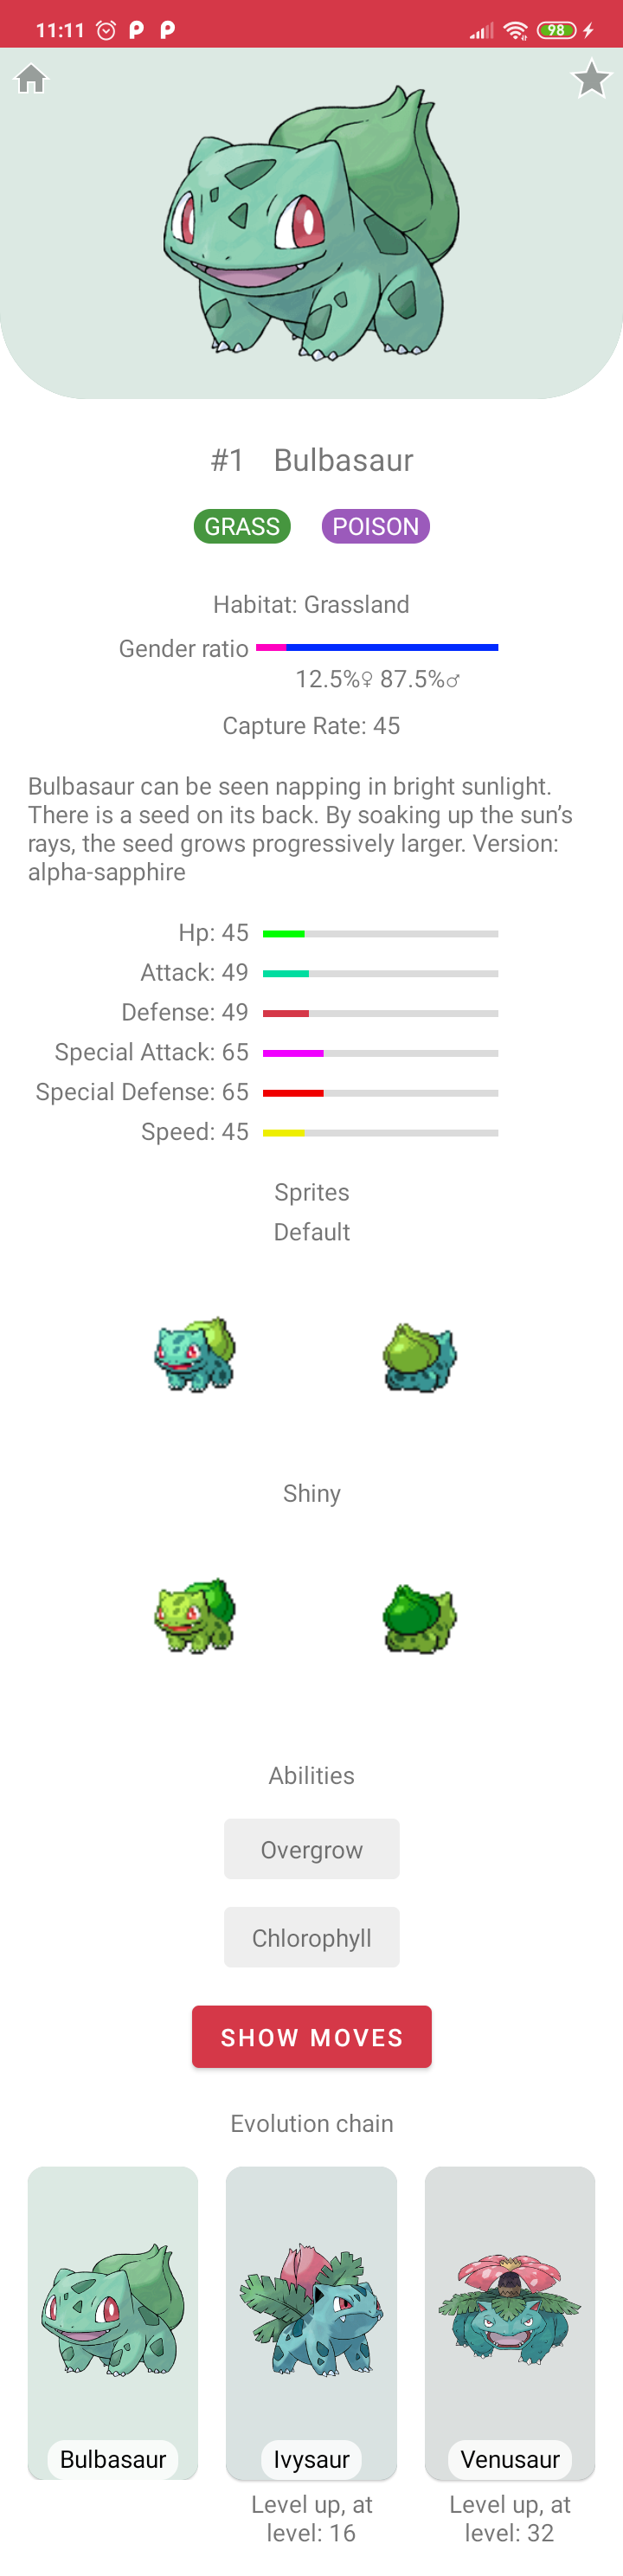
\includegraphics[width=150px]{detail.png}}
	\caption{Dettagli del Pokémon.}
\end{figure}

\newpage

\subsection{Mosse ed Abilità}
\paragraph{Mosse}
Il bottone per mostrare le mosse è cliccabile. Al click, mostra una schermata con tutte le mosse che il Pokémon può apprendere. Vengono mostrati nome, metodo di apprendimento, tipo di danno e tipo della mossa.\\
Le mosse sono cliccabili. Al click, la carta si espande e, dopo un breve caricamento delle informazioni dall’API, mostra informazioni aggiuntive della mossa, quali: Potenza, Precisione, PP e testo di descrizione.

\paragraph{Abilità}
Le abilità sono cliccabili. Al click, dopo un breve caricamento delle informazioni dall’API, vengono mostrati i dettagli dell’abilità.\\
\begin{figure}[h!]
  \fbox{\centering
  \begin{subfigure}[b]{0.3\linewidth}
    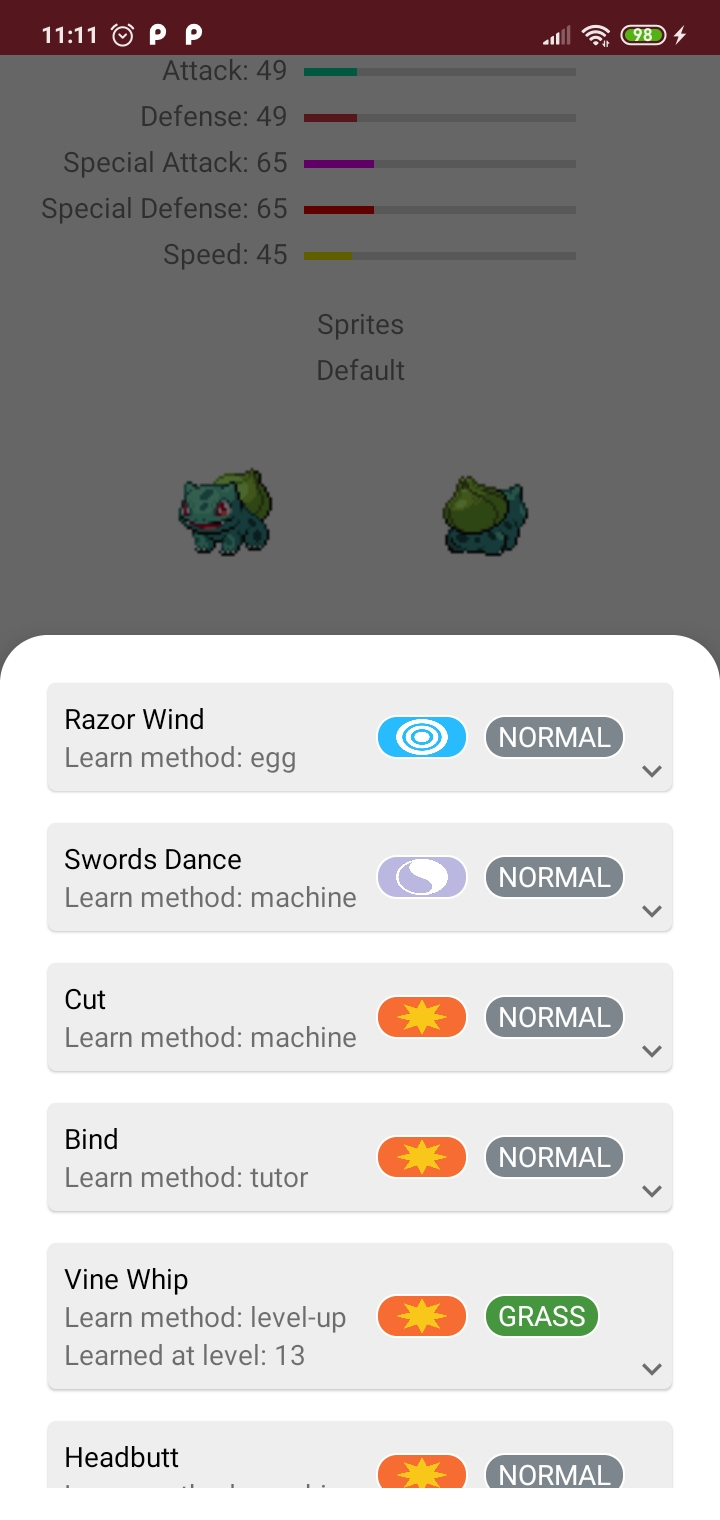
\includegraphics[width=\linewidth]{moves.jpg}
    \caption{List Mosse.}
  \end{subfigure}
  \begin{subfigure}[b]{0.3\linewidth}
    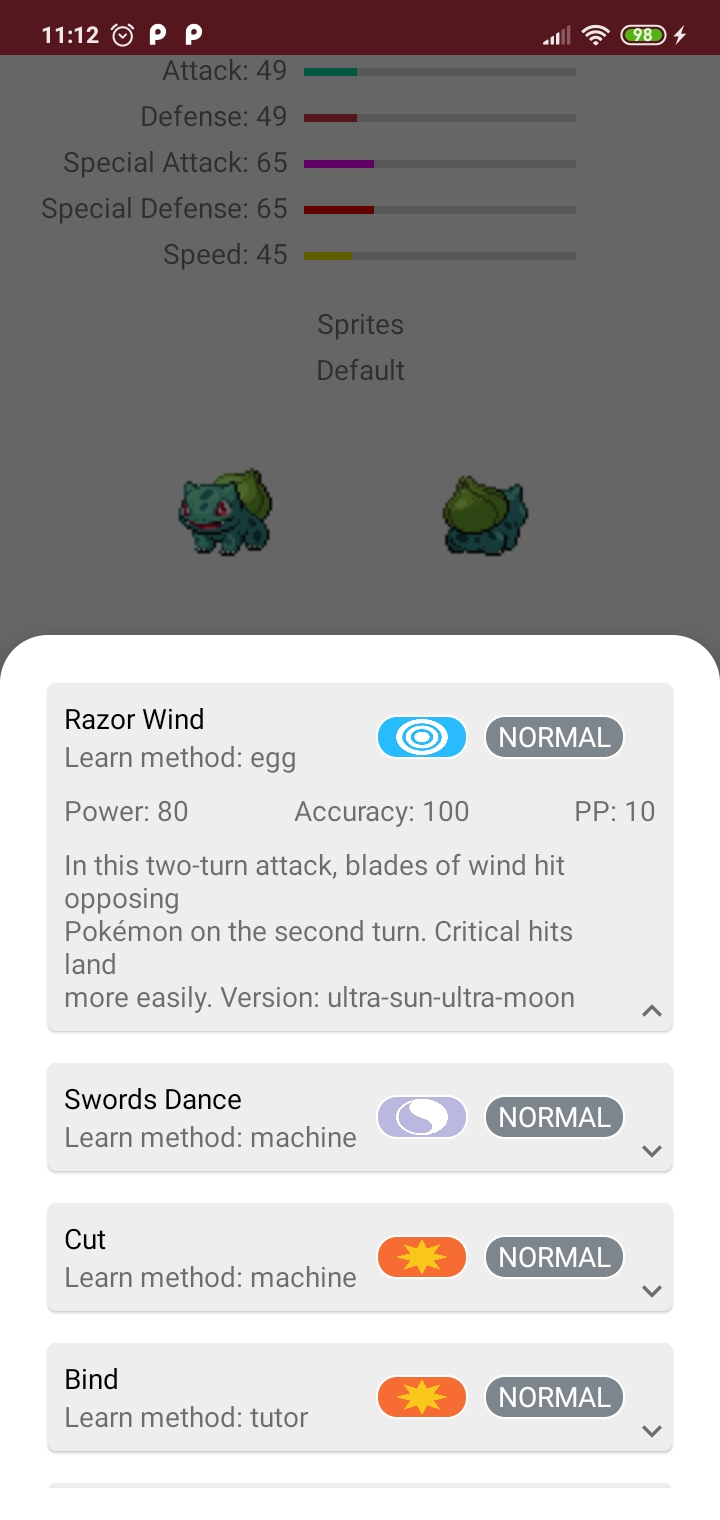
\includegraphics[width=\linewidth]{moves_expansion.jpg}
    \caption{Dettagli mossa.}
  \end{subfigure}
    \begin{subfigure}[b]{0.3\linewidth}
    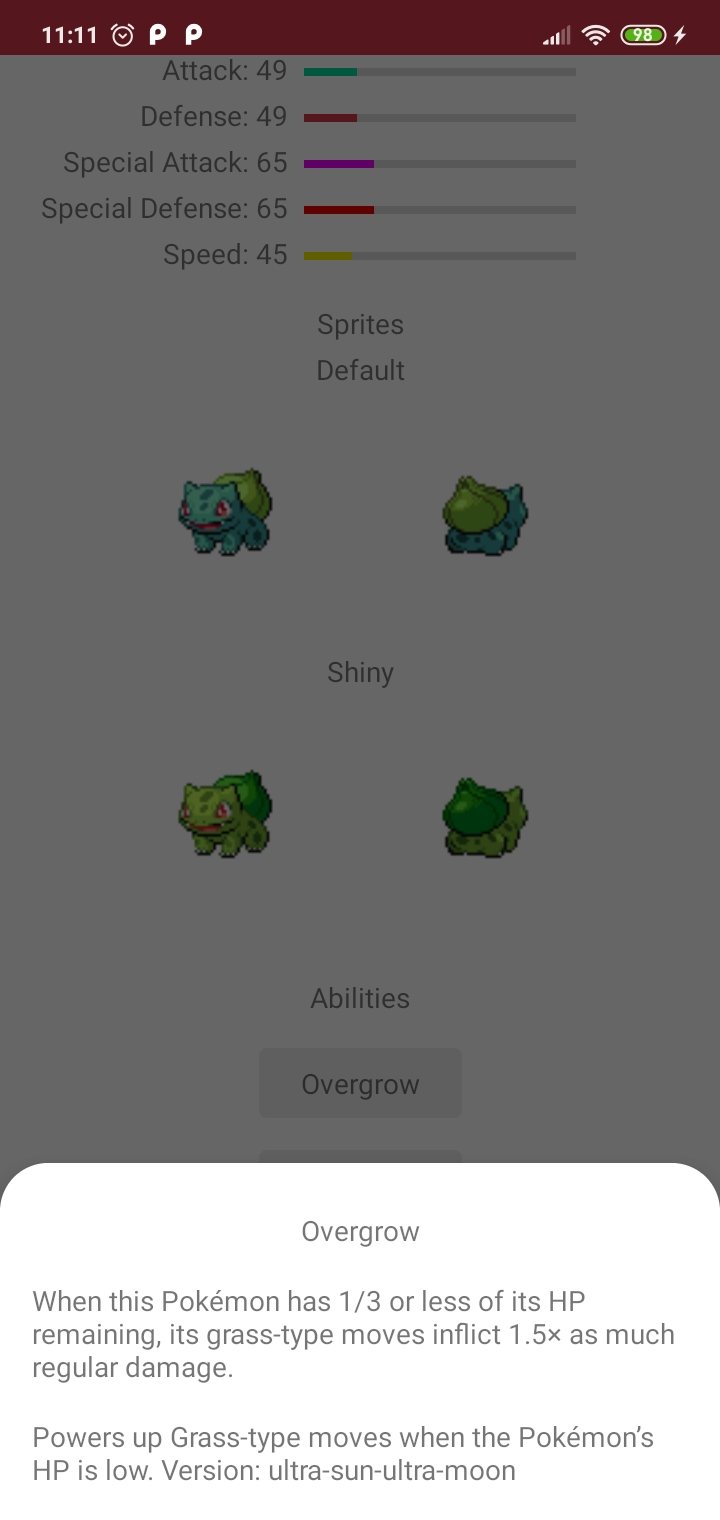
\includegraphics[width=\linewidth]{ability.jpg}
    \caption{Dettagli Abilità.}
  \end{subfigure}}
\end{figure}
\newpage

\section{Who’s that pokemon?}
  All’apertura della schermata, e ad ogni cambio di Pokémon, viene riprodotta la traccia audio del tema del minigioco.\\
Lo scopo del mini gioco è indovinare il nome del Pokémon data la sua sagoma oscurata.\\
Il nome del Pokémon va inserito nell’apposito campo.\\
Se al click del bottone “Conferma” il nome è corretto, la sagoma del Pokémon viene sostituita dall’immagine colorata di questo.\\
Il bottone “Rivela” permette di rivelare nome e immagine del Pokémon anche se non lo si conosce.\\
Il bottone “Prossimo” genera casualmente un nuovo Pokémon.\\

\begin{figure}[h!]
  \fbox{\centering
  \begin{subfigure}[b]{0.4\linewidth}
    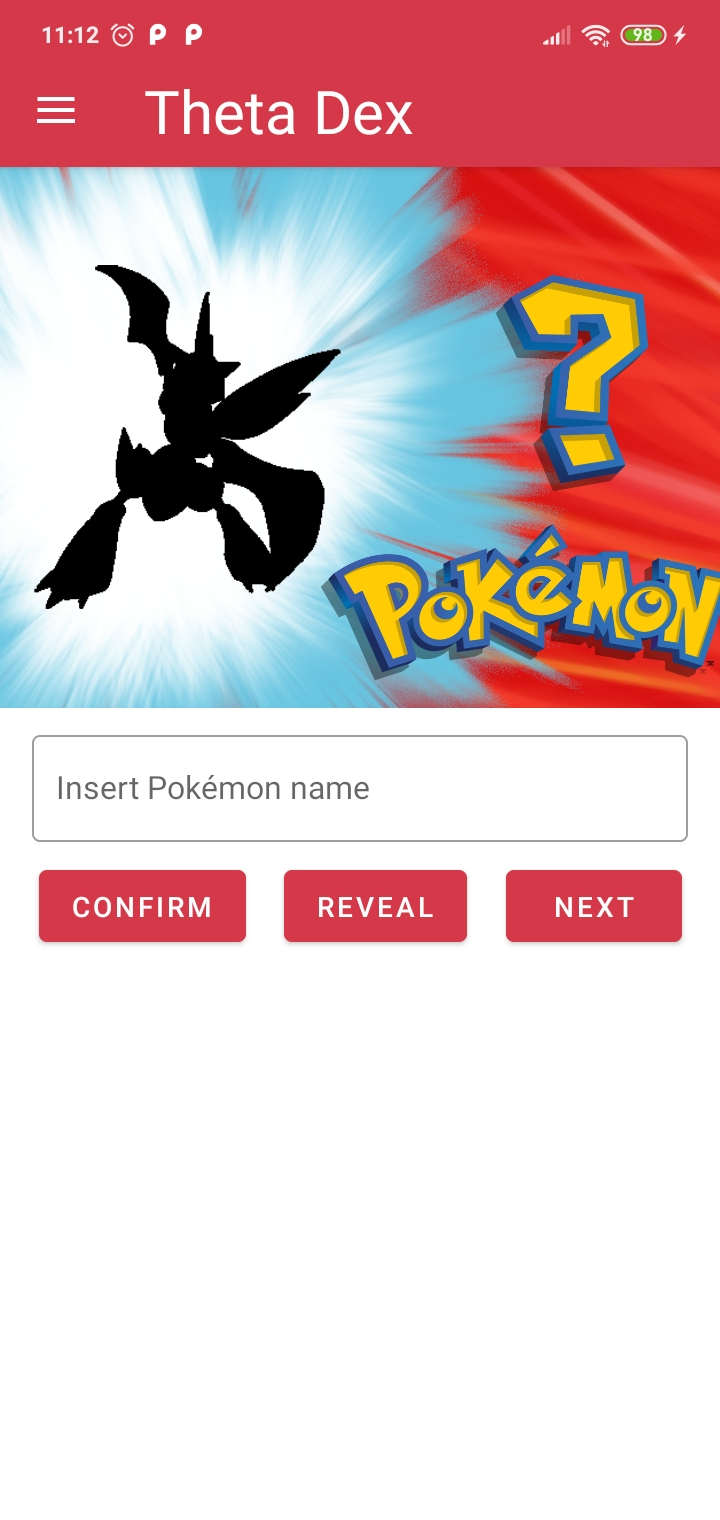
\includegraphics[width=\linewidth]{who.jpg}
    \caption{Gioco.}
  \end{subfigure}
  \begin{subfigure}[b]{0.4\linewidth}
    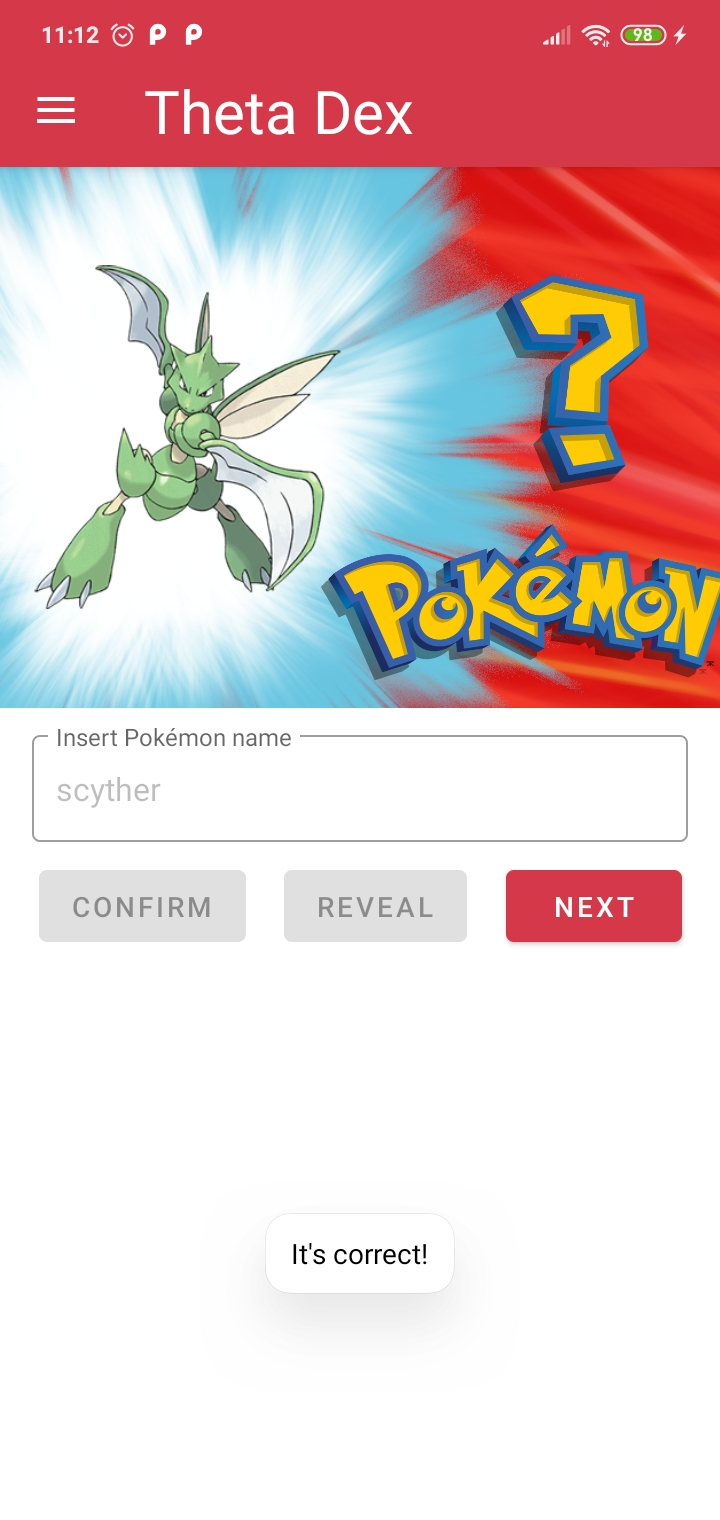
\includegraphics[width=\linewidth]{who_correct.jpg}
    \caption{Pokemon Indovinato.}
  \end{subfigure}
  }
\end{figure}
\newpage

  \section{Impostazioni}
  Qui si possono cambiare le impostazioni dell’applicazione.\\
Si può decidere se utilizzare il tema chiaro, scuro o quello utilizzato dal sistema Android.\\
Si possono cancellare i dati dell’applicazione. Ciò farà chiudere l’applicazione, ed al successivo avvio sia avrà nuovamente la fase di inizializzazione come al primo avvio.\\
Si può scegliere se attivare o disattivare il volume dell’applicazione. Ciò influenza il minigioco “Who’s that Pokémon?”.\\
  \begin{figure}[h!]
    \centering
  \fbox{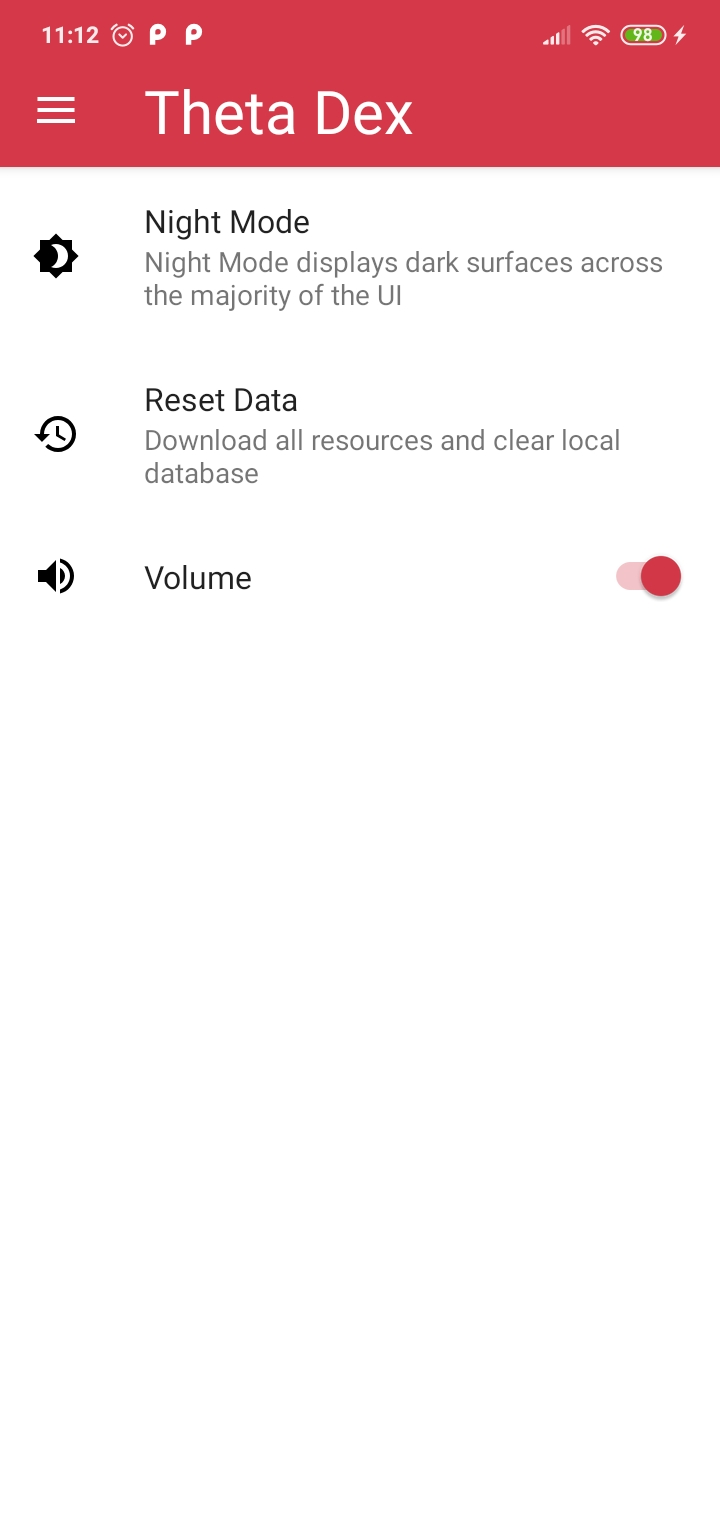
\includegraphics[width=150px]{setting.jpg}}
  \caption{Schermata caricamento iniziale.}
\end{figure}
\newpage

\section{Informazioni}
Schermata in cui sono rappresentati gli sviluppatori dell’applicazione ed il logo dell’API che viene utilizzata.
  \begin{figure}[h!]
    \centering
  \fbox{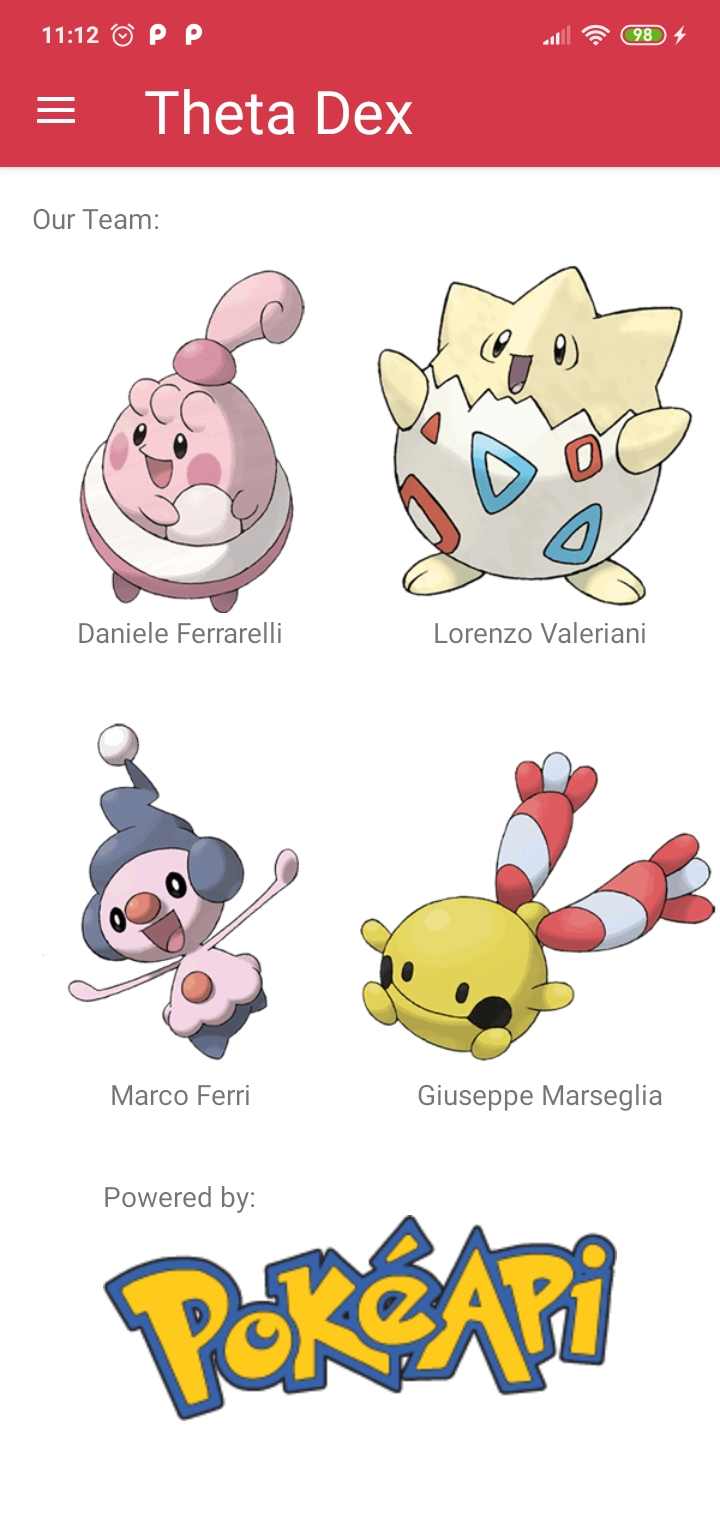
\includegraphics[width=150px]{about.jpg}}
  \caption{Schermata caricamento iniziale.}
\end{figure}
\end{document}